\documentclass[a4paper,12pt]{report}
\usepackage[a4paper,left=3cm,right=2cm,top=2.5cm,bottom=2.5cm]{geometry}
\usepackage[utf8]{inputenc}
\usepackage{graphicx}
\usepackage[table]{xcolor}
\usepackage{array}
\usepackage{float}
\usepackage{hyperref}
\hypersetup{hidelinks}
\usepackage{amsmath}
\usepackage[ruled,vlined,linesnumbered,algoruled]{algorithm2e}
\usepackage{tabularx}

% Define subsubsubsection
\makeatletter
\newcounter{subsubsubsection}[subsubsection]
\renewcommand\thesubsubsubsection{\thesubsubsection.\@arabic\c@subsubsubsection}
\newcommand\subsubsubsection{\@startsection{subsubsubsection}{4}{\z@}%
									 {-3.25ex\@plus -1ex \@minus -.2ex}%
									 {1.5ex \@plus .2ex}%
									 {\normalfont\normalsize\bfseries}}
\newcommand*{\subsubsubsectionmark}[1]{}
\makeatother

% Dades de la pràctica
\newcommand{\titolPractica}{Supermaket Manager}
\newcommand{\identificadorEquip}{Subrgrup 11.3}
\newcommand{\PROPquatrimestre}{PROP - Quadrimestre de tardor 2024}
\newcommand{\versioLliurament}{Versió del lliurament 1.0}

% Dades de renovar comandes
\renewcommand*\contentsname{Continguts}
\renewcommand{\figurename}{Figura}
\renewcommand{\tablename}{Taula}

\begin{document}

% Tapa del document
\begin{titlepage}
	\begin{center}
		{\Large \textbf{\titolPractica}} \\[10cm]
		\textbf{\large \identificadorEquip} \\[1cm]
		Guillem Cabré Farré, \small{@guillem.cabre} \\
		Marc Peñalver Guilera, \small{@marc.penalver} \\
		Àlex Rodríguez Rodríguez, \small{@alex.rodriguez.r} \\
		Marc Teixidó Sala, \small{@marc.teixido} \\[2cm]
		\textbf{\versioLliurament} \\
		\textbf{\PROPquatrimestre} \\
		\textbf{Data: \today}
	\end{center}
\end{titlepage}

% Índex de continguts
\tableofcontents
\clearpage

\chapter{Definició de classes i les seves estructures de Dades}

\section{Classes, interfícies i enums}

Per al desenvolupament d'aquest projecte, hem decidit utilitzar un conjunt de classes i interfícies que ens permetin implementar de manera eficient els diferents casos d'ús que hem dissenyat. Aquestes classes no només es fonamenten en les funcionalitats essencials per al bon funcionament de l'aplicació, sinó que també segueixen els principis i patrons de disseny orientat a objectes per assegurar una bona qualitat de codi i facilitat d'ampliació. \\

Un dels principis fonamentals que hem adoptat en el disseny de les nostres classes és el **principi obert-tancat** (\textit{Open-Closed Principle}), el qual estableix que una classe hauria d'estar oberta per a l'extensió, però tancada per a la modificació. Això vol dir que podem afegir noves funcionalitats a través de l'extensió de classes existents o la implementació de noves interfícies, sense necessitat de modificar el codi ja existent. D'aquesta manera, garantim que el sistema sigui altament mantenible i escalable, facilitant la incorporació de noves característiques sense alterar la base del sistema ja implementat.\\

A continuació, es detallen les principals classes i interfícies que hem dissenyat, les quals formen l'estructura fonamental del projecte. Aquestes classes estan dissenyades per ser reutilitzades i adaptades a les diferents necessitats que poden sorgir a mesura que el projecte creixi i es modifiqui.

\begin{itemize}
	\item \textbf{Classe \texttt{Supermarket}}:
	      \begin{itemize}
		      \item \textbf{Descripció:} Representa la distribució d'un supermercat, com a un conjunt de prestatgeries amb productes. Aquesta classe serà de tipus \textit{singleton}, d'aquesta manera serà accessible en tot moment i només hi haurà una instància d'aquesta en tot el programa.
		      \item \textbf{Estructures de dades:}
		            \begin{itemize}
			            \item \texttt{instance} (Supermarket): Instància d'ella mateixa per poder agafar-la des de qualsevol lloc del codi.
			            \item \texttt{registeredUsers} (ArrayList(Users)): Llista d'usuaris del supermercat.
			            \item \texttt{logedUser} (User): Usuari que té la sessió iniciada.
			            \item \texttt{shelvingUnits} (ArrayList(ShelvingUnit)): Llista d'unitats d'emmagatzematge.
			            \item \texttt{shelvingUnitHeigth} (int): Alçada de les prestatgeries.
			            \item \texttt{orderingStrategy} (OrderingStrategy): Estrategia d'ordenació.
			            \item \texttt{importFileStrategy} (ImportFileStrategy): Estrategia d'importació.
			            \item \texttt{exportFileStrategy} (ExportFileStrategy): Estrategia d'exportació.
			            \item \texttt{ADMIN-NAME} (String): Nom d'usuari de l'administrador.
			            \item \texttt{ADMIN-PASSWORD} (String): Contrasenya de l'administrador.
			            \item \texttt{EMPLOYEE-NAME} (String): Nom d'usuari de tots els empleats.
			            \item \texttt{EMPLOYEE-PASSWORD} (String): Contrasenya de tots els empleats.
		            \end{itemize}
	      \end{itemize}
	\item \textbf{Classe \texttt{ShelvingUnit}}:
	      \begin{itemize}
		      \item \textbf{Descripció:} Representa una unitat d'emmagatzematge "prestatgeria" en un supermercat, on s'emmagatzemen un determinat tipus de productes en diferents alçades.
		      \item \textbf{Estructures de dades:}
		            \begin{itemize}
			            \item \texttt{uid} (Enter): Identificador únic per a la prestatgeria.
			            \item \texttt{products} (List(Product)): Llista que conté els productes de la prestatgeria ordenats per alçades.
			            \item \texttt{temperature} (ProductTemperature): Temperatura que proporciona la prestatgeria per emmagatzemar els productes que necessitin aquella temperatura.
		            \end{itemize}
	      \end{itemize}
	\item \textbf{Classe \texttt{Product}}:
	      \begin{itemize}
		      \item \textbf{Descripció:} Representa un producte dins del sistema, amb els atributs essencials.
		      \item \textbf{Estructures de dades:}
		            \begin{itemize}
			            \item \texttt{name} (String): Nom del producte.
			            \item \texttt{price} (float): Preu del producte.
			            \item \texttt{temperature} (ProductTemperature): Temperatura necessitada per emmagatzemar el producte.
			            \item \texttt{keyWords} (List(String)): Paraules clau associades al producte per fer busquedes.
			            \item \texttt{relatedProducts} (List(RelatedProduct)): Llista que mostra tots els productes relacionats amb ell junt amb el seu grau de relació.
		            \end{itemize}
	      \end{itemize}
	\item \textbf{Classe \texttt{RelatedProduct}}:
	      \begin{itemize}
		      \item \textbf{Descripció:} Gestiona la relació d'un producte amb un altre amb un grau de relació anomenat similitud.
		      \item \textbf{Estructures de dades:}
		            \begin{itemize}
			            \item \texttt{value} (float): Grau de similitud dels dos productes.
			            \item \texttt{product1} (Product): Primer producte de la relació. No pot ser null.
			            \item \texttt{product2} (Product): Segon producte de la relació. Diferent al primer i no pot ser null.
		            \end{itemize}
	      \end{itemize}
	\item \textbf{Enum \texttt{ProductTemperature}}:
	      \begin{itemize}
		      \item \textbf{Descripció:} Enum per gestionar les temperatures de emmagatzematge recomanades per a productes que necessiten condicions específiques de temperatura.
	      \end{itemize}
	\item \textbf{Classe \texttt{Catalog}}:
	      \begin{itemize}
		      \item \textbf{Descripció:} Gestiona una col·lecció de productes, proporcionant mètodes per afegir, eliminar i cercar a través de l' inventari disponible.
		      \item \textbf{Estructures de dades:}
		            \begin{itemize}
			            \item \texttt{catalog} (Catalog): Instancia del catàleg per poder usar-lo en qualsevol lloc del codi.
			            \item \texttt{products} (List(Product)): Col·lecció de tots els productes al catàleg.
		            \end{itemize}
	      \end{itemize}
	\item \textbf{Classe \texttt{ImportFileJSON}}:
	      \begin{itemize}
		      \item \textbf{Descripció:} Classe per importar arxius JSON que contenen dades de productes i informació relacionada.
	      \end{itemize}
	\item \textbf{Classe \texttt{ExportFileJSON}}:
	      \begin{itemize}
		      \item \textbf{Descripció:} Classe per exportar configuracions a arxius JSON que contenen dades de productes i informació relacionada.
	      \end{itemize}
	\item \textbf{Classe \texttt{Approximation}}:
	      \begin{itemize}
		      \item \textbf{Descripció:} Classe per implementar el algorisme d'ordenació per aproximació.
	      \end{itemize}
	\item \textbf{Classe \texttt{BruteForce}}:
	      \begin{itemize}
		      \item \textbf{Descripció:} Classe per implementar el algorisme d'ordenació per força bruta.
	      \end{itemize}
	\item \textbf{Interfície \texttt{OrderingStrategy}}:
	      \begin{itemize}
		      \item \textbf{Descripció:} Interfície per a estratègies d'ordenació del supermercat per decidir quin algorisme es fa servir.
	      \end{itemize}
	\item \textbf{Interfície \texttt{ImportFileStrategy}}:
	      \begin{itemize}
		      \item \textbf{Descripció:} Interfície per a estratègies d'importació de fitxers, permetent la importació de dades des de diferents formats de fitxer.
	      \end{itemize}
	\item \textbf{Interfície \texttt{ExportFileStrategy}}:
	      \begin{itemize}
		      \item \textbf{Descripció:} Interfície per a estratègies d'exportació de fitxers, permetent l'exportació de dades en diversos formats.
	      \end{itemize}
\end{itemize}

\section{Relació de classes}

A la següent taula es mostra com es distribuirà el treball entre els membres de l’equip. Cada membre té assignades diverses classes amb els seus tests unitaris respectius. En el cas de la classe \texttt{Supermarket}, aquesta s’ha dividit entre dos membres. A continuació s’especifica com es durà a terme aquesta divisió.

\begin{table}[H]
	\centering
	\setlength{\arrayrulewidth}{0.5mm}
	\setlength{\tabcolsep}{5pt}
	\renewcommand{\arraystretch}{1.5}
	\arrayrulecolor{black}
	\centering
		\begin{tabularx}{\textwidth}{|X|X|X|X|} % X ajusta automáticamente las columnas al ancho
			\hline
			\rowcolor{gray!40} % Fila de encabezado con fondo gris claro
			guillem.cabre            & marc.penalver      & alex.rodriguez.r & marc.teixido    \\
			\hline
			Catalog                  & Supermarket        & OrderingStrategy & Supermarket     \\
			\hline
			ShelvingUnit             & User               & BruteForce       & DomainController\\
			\hline
			Product                  & Admin              & Approximation    & Javadoc         \\
			\hline
			RelatedProduct           & ExportFileStrategy & Greedy           & \LaTeX          \\
			\hline
			ProductTemperat-\newline ure       & ImportFileStrategy & DomainController & DomainController-\newline Driver \\
			\hline
			ExportFileJSON           & DomainController   & \LaTeX           & Tests d'integració \\
			\hline
			ImportFileJSON           & DomainController-\newline Driver & DomainController-\newline Driver & \\
			\hline
			SupermarketData          &                    &                  &                 \\
			\hline
			RelatedProduct-\newline Serializer &                    &                  &                 \\
			\hline
		\end{tabularx}
	\end{table}

En marc.penalver ha realizat les funcionalitats relacionades amb els usuaris, crida a les estrategies d'ordenació i gestió de fitxers. D'altra banda, en marc.teixido ha realizat les funcionalitats relacionades amb les \texttt{ShelvingUnits}.

\section{Estructura JSON}

El fitxer JSON utilitzat en l'aplicació ``Supermarket Manager'' emmagatzema la informació relacionada amb els productes disponibles al supermercat, així com la distribució d'aquests en els prestatges. Aquest fitxer conté els elements següents:

\begin{itemize}
	\item \textbf{shelvingUnitHeight}: Representa l'alçada en unitats per als prestatges del supermercat. És un enter que indica el nombre de files que pot tenir cada prestatgeria.

	\item \textbf{products}: Aquesta és una llista que conté informació detallada sobre cada producte disponible al supermercat. Cada producte té els atributs següents:
	      \begin{itemize}
		      \item \textbf{name}: El nom del producte.
		      \item \textbf{price}: El preu del producte, expressat com un nombre decimal.
		      \item \textbf{temperature}: La temperatura de conservació necessària per al producte, que pot ser \textit{AMBIENT}, \textit{REFRIGERATED} o \textit{FROZEN}.
		      \item \textbf{imgPath}: La ruta relativa de la imatge associada al producte.
		      \item \textbf{keyWords}: Una llista de paraules clau que descriuen el producte i permeten una cerca més eficient.
		      \item \textbf{relatedProducts}: Una llista de relacions amb altres productes. Cada relació conté:
		            \begin{itemize}
			            \item \textbf{value}: Un valor numèric que indica el grau de relació entre dos productes (per exemple, en termes de complementarietat).
			            \item \textbf{product1} i \textbf{product2}: Els noms dels productes que estan relacionats.
		            \end{itemize}
	      \end{itemize}

	\item \textbf{distribution}: Aquesta és una llista que defineix la distribució dels productes en els diferents prestatges del supermercat. Cada entrada d'aquesta llista té els atributs següents:
	      \begin{itemize}
		      \item \textbf{uid}: Un identificador únic per al prestatge.
		      \item \textbf{height}: L'alçada del prestatge, que defineix quantes files té.
		      \item \textbf{temperature}: La temperatura requerida per al prestatge, que pot ser \textit{AMBIENT}, \textit{REFRIGERATED} o \textit{FROZEN}.
		      \item \textbf{products}: Una llista que conté els noms dels productes col·locats en les diferents posicions del prestatge. Si un espai està buit, es representa amb un valor \texttt{null}.
	      \end{itemize}
\end{itemize}

Aquest fitxer JSON és fonamental per mantenir la configuració del supermercat quan es tanca l'aplicació, ja que permet carregar tant el catàleg de productes com la seva distribució de forma eficaç en reobrir el programa.


\chapter{Algorismes per a la distribució de productes al Supermercat}

\section{Introducció}

Al supermercat s'ha vist que al col·locar certs productes seguits d'altres els clients tendeixen a comprar-los junts i, per tant, augmenten les vendes del supermercat.
És per aquest motiu que s'han decidit implementar tres algorismes que permetin distribuir els productes a les prestatgeries de manera que aquestes relacions es maximitzin i, per tant, que així ho facin, també, els beneficis de la botiga.

\section{Objectiu}
El problema a resoldre consisteix en:
\begin{itemize}
	\item Col·locar el màxim de productes \(P = \{p_1, p_2, \dots, p_m\}\) possibles en les prestatgeries \(S = \{s_1, s_2, \dots, s_n\}\).
	\item Respectar les restriccions de temperatura de cada prestatgeria i producte: un producte només es pot col·locar en una prestatgeria si la seva temperatura és compatible amb la de la prestatgeria.
	\item Maximitzar la \textbf{puntuació total}, que es defineix com la suma de les \textbf{similituds} entre productes consecutius:
	      \[
		      \text{Puntuació total} = \sum_{i=1}^{k-1} \text{similitud}(p_i, p_{i+1}),
	      \]
	      on \(k\) és el nombre de productes col·locats.
\end{itemize}

\section{Organització de les prestatgeries}

El supermercat està organitzat en prestatgeries d'una alçada fixa \( h \), idèntica per a totes les prestatgeries. Cada prestatgeria es pot considerar com una columna que emmagatzema productes, on la \textbf{primera posició} correspon al nivell més alt i la \textbf{darrera posició} al nivell més baix.

No obstant, si considerem la visió global del supermercat, aquest es pot representar com una única llista \textbf{ciclíca} de poiscions, tal i com es pot veure a la figura 2.1. Per recorrer la llista es va horitzontalment fins a arribar a la prestatgeria inicial o final i quan s'arriba a aquest punt es baixa o puja una posició, respectivament.
D'aquesta manera, el \textbf{nombre total de posicions} on es poden col·locar productes ve donat per la fórmula:
\[
	\textit{Nombre total de posicions} = n \times h
\]
on \( n \) és el nombre de prestatgeries i \( h \) l'alçada de cadascuna.

\subsection{Adreçament de les prestatgeries i les posicions dels productes}

Per identificar a quina prestatgeria pertany un producte, utilitzem la seva posició \( i \) dins la llista. Això es calcula amb l'expressió:
\[
	\textit{Prestatgeria actual} = i \bmod n
\]
on \( i \) és la posició del producte en la llista.
\newline
D'altra banda, per accedir al nivell d'alçada del producte dins de la prestatgeria, fem servir la fórmula següent:
\[
	\textit{Alçada actual} = h - 1 - \left\lfloor \frac{i}{n} \right\rfloor
\]

Aquesta estructuració permet indexar els productes de manera eficient i mantenir una representació unificada del supermercat tant com una llista global com des de la perspectiva de cada prestatgeria.


\begin{figure}[H]
	\centering
	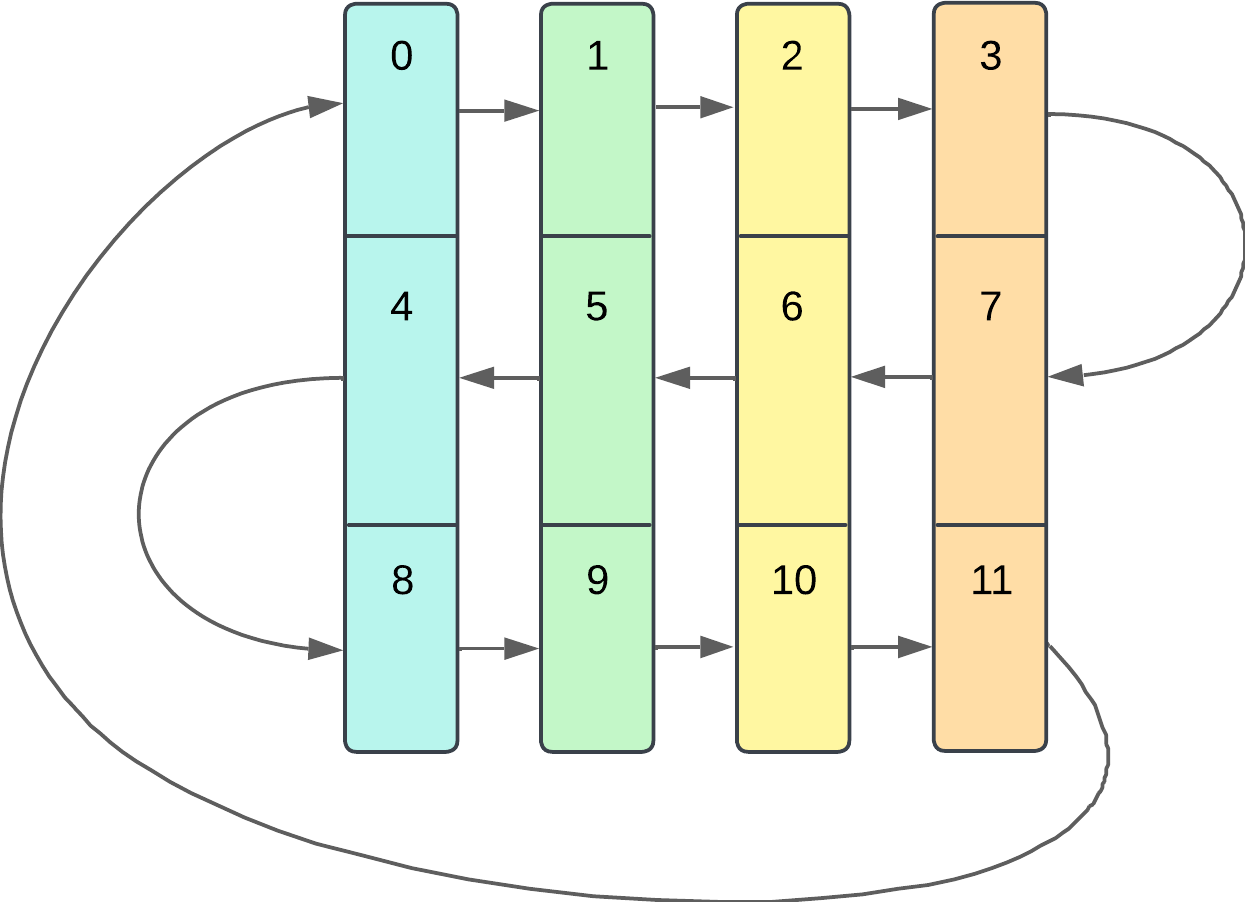
\includegraphics[width=0.75\textwidth]{../assets/shelvingUnit_array_diagram.png}
	\caption{Recorregut de les prestatgeries en els algorismes}
\end{figure}

A continuació, es descriuran els tres diferents algorismes implementats per a la distribució de productes al supermercat.

\section{Algorisme de força bruta}

Aquest algorisme, definit a la classe \texttt{BruteForce}, utilitza una estratègia de \textbf{backtracking} per trobar la distribució òptima dels productes en les prestatgeries del supermercat. L'objectiu és maximitzar una funció de \textbf{puntuació total}, que considera la similitud entre productes col·locats consecutivament i l'eficiència en l'ús de l'espai.

\subsection{Pseudocodi de l'algorisme}
L'algorisme està dividit en dues parts principals: una funció principal que inicialitza els paràmetres i una funció recursiva que col·loca els productes fent servir \textbf{backtracking}.
\newline
\begin{algorithm}[H]
	\SetAlgoVlined
	\caption{Col·locació òptima de productes amb força bruta}
	\KwIn{Prestatgeries $S$, productes $P$}
	\KwOut{Distribució òptima $S^*$}
	$highestScore \gets -1$, $optimalDistribution \gets S$\;

	\For{$i = 0$ \textbf{fins a} $n \times h$}{
		$shelf \gets S[i \bmod n]$\;
		\For{$p \in P$}{
			\If{$shelf$ pot emmagatzemar $p$}{
				Afegir $p$ a $shelf$\; 
				Crida recursiva amb $nextIndex$\;
				Desfer col·locació de $p$\;
			}
		}
	}
	\Return $optimalDistribution$\;

	\

	\SetKwFunction{FuncRecursivelyPlaceProducts}{recursivelyPlaceProducts}
	\FuncRecursivelyPlaceProducts{$i, P, S, prev, score$}{

		\If{$P$ buida \textbf{o} $i \geq n \times h$}{
			\If{$score > highestScore$}{
				$highestScore \gets score$, $optimalDistribution \gets S$\;
			}
			\Return\;
		}

		$shelf \gets S[i \bmod n]$, $height \gets h - 1 - \left\lfloor \frac{i}{n} \right\rfloor$;
		\For{$c \in P$}{
			\If{$shelf$ pot emmagatzemar $c$}{
				Afegir $c$ a $shelf$\;
				Crida recursiva amb $nextIndex$\;
				Desfer col·locació de $c$\;
			}
		}
	}
\end{algorithm}




\subsection{Complexitat}
L'algorisme \textbf{BruteForce} utilitza una estratègia de \textbf{backtracking} per trobar la distribució òptima dels productes a les prestatgeries. La seva complexitat depèn del nombre de prestatgeries (\(n\)), de l'alçada de les prestatgeries (\(h\)) i del nombre de productes (\(m\)).

\subsubsection{Funció principal (\texttt{orderSupermarket})}

La funció principal itera sobre totes les posicions possibles del supermercat (\(n \times h\)) i, per cada posició, comprova tots els productes disponibles (\(m\)). Això dona una complexitat inicial de:

\[
O(n \times h \times m)
\]

\subsubsection{Recursió (\texttt{recursivelyPlaceProducts})}

En cada pas de la recursió:
\begin{itemize}
    \item \textbf{Exploració de totes les combinacions:} Aquest algoritme prova totes les combinacions possibles de col·locació de productes. Això implica que la recursió pot explorar totes les permutacions dels \(m\) productes, la qual cosa té una complexitat de \(O(m!)\).
    \item \textbf{Comprovació de compatibilitat:} Per cada producte candidat, es comprova si és compatible amb la prestatgeria actual. Aquesta operació es fa \(m\) vegades per cada pas de la recursió, afegint un factor multiplicatiu de \(O(m)\) a cada pas.
\end{itemize}

La complexitat total de la recursió és, per tant:

\[
O(m \times m!) = O((m+1)!)
\]

\subsubsection{Poda}

L'algorisme utilitza estratègies de poda per evitar explorar configuracions innecessàries. Les principals estratègies són:
\begin{itemize}
    \item \textbf{Poda basada en la puntuació:} Si la puntuació màxima possible d'una configuració no supera la millor puntuació registrada, es descarta aquesta branca de l'exploració.
    \item \textbf{Compatibilitat:} Només es consideren productes que són compatibles amb la prestatgeria actual.
\end{itemize}

Tot i això, en el pitjor cas, la poda no pot evitar explorar totes les permutacions possibles.

\subsubsection{Complexitat global}

Combinant els costos de la funció principal i la recursió, la complexitat global en el pitjor cas és:

\[
O(n \times h \times m \times m!)
\]

\subsubsection{Resum}

\begin{itemize}
    \item \textbf{Pitjor cas teòric:} \(O(n \times h \times m \times m!)\)
    \item \textbf{Millor cas pràctic:} En situacions on la poda és efectiva (per exemple, amb una forta restricció de compatibilitat), l'espai de cerca es redueix significativament, però segueix sent exponencial en funció de \(m\).
    \item \textbf{Quan fer-lo servir:} Aquest algorisme és adequat per conjunts de productes petits o amb una forta relació entre productes, ja que en aquests casos la poda pot reduir significativament l'espai de cerca.
\end{itemize}


\section{Algorisme Greedy}

L'algorisme Greedy, implementat a la classe \texttt{GreedyBacktracking}, segueix una estratègia de \textbf{selecció de productes} basada en la similitud entre productes consecutius. Aquest algorisme busca maximitzar la puntuació total de la distribució, però no garanteix una solució òptima.
\newline
L'estrategia que segueix és semblant a la de l'algorisme de força bruta, amb la diferència que en cada pas, selecciona el producte que \textbf{millor similitud} té amb el producte col·locat a la posició anterior a l'actual, en comptes de provar totes les combinacions possibles.

\subsection{Pseudocodi de l'algorisme}

La part diferencial de l'algorisme respecte al \texttt{BruteForce} es troba en la funció \texttt{findBestProductToPlace}, que selecciona el producte amb la millor similitud amb el producte anterior. 
Aquesta funció retorna el producte seleccionat i la similitud associada.
\newline
\begin{algorithm}[H]
	\SetAlgoVlined
	\caption{Col·locació òptima amb backtracking greedy}
	\SetKwFunction{FuncFindBestProductToPlace}{findBestProductToPlace}
	\FuncFindBestProductToPlace{$i$, $P$, $S$, $prev$}{
		$shelf \gets S[i \bmod n]$\;
		$bestProduct \gets$ null, $bestSimilarity \gets 0$\;
		\ForEach{$p \in P$}{
			\If{$shelf$ pot emmagatzemar $p$}{
				$similaritat \gets$ similitud($prev$, $p$)\;
				\If{$similaritat > bestSimilarity$}{
					$bestSimilarity \gets similaritat$\;
					$bestProduct \gets p$\;
				}
			}
		}
		\Return{$(bestProduct, bestSimilarity)$}\;
	}
\end{algorithm}

\subsection{Complexitat}

La funció principal itera sobre totes les posicions possibles del supermercat (\(n \times h\)) i, per cada posició, comprova tots els productes disponibles (\(m\)). Això dona una complexitat inicial de:

\[
O(n \times h \times m)
\]

\subsubsection{Recursió (\texttt{recursivelyPlaceProducts})}

En cada pas de la recursió:
\begin{itemize}
    \item \textbf{Selecció del millor producte:} Es fa mitjançant la funció \texttt{findBestProductToPlace}, que revisa tots els productes restants (\(m\)) per seleccionar el millor. Això té una complexitat de \(O(m)\).
    \item \textbf{Crides recursives:} L'algorisme pot fer fins a \(m\) crides recursives, ja que cada producte es col·loca una vegada. En el pitjor cas, es podrien explorar totes les configuracions possibles de col·locació.
\end{itemize}

Per tant, el cost de la recursió en el pitjor cas és:

\[
O(m!)
\]

\subsubsection{Poda}

L'algorisme incorpora una estratègia de \textbf{poda greedy} per evitar explorar configuracions poc prometedores. Això redueix el nombre de configuracions explorades en la pràctica, però no elimina el factor \(m!\) en el pitjor cas, ja que encara podria caldre explorar totes les opcions en escenaris adversos (per exemple, si la similitud entre productes és molt baixa i cal provar totes les opcions).

Combinant els costos de la funció principal i la recursió, tenim la següent complexitat global en el pitjor cas:

\[
O(n \times h \times m \times m!)
\]

En la pràctica, gràcies a la poda, la complexitat es redueix significativament, tot i que encara és considerable. La complexitat efectiva depèn de:
\begin{itemize}
    \item \textbf{Qualitat de la poda:} Si molts productes són incompatibles o si les puntuacions màximes es descarten ràpidament, es redueixen les configuracions explorades.
    \item \textbf{Compatibilitat dels productes amb les prestatgeries:} Si molts productes no són compatibles amb certes prestatgeries, l'espai de cerca també es redueix.
\end{itemize}

\subsubsection{Resum}

\begin{itemize}
    \item \textbf{Pitjor cas teòric:} \(O(n \times h \times m \times m!)\)
    \item \textbf{Millor cas pràctic:} \(O(n \times h \times m^2)\), si només es consideren un nombre limitat de configuracions viables gràcies a la poda.
\end{itemize}

Aquest algorisme és més eficient que un de força bruta pur (\(O((n \times h \times m)!)\)), però encara és costós per a valors grans de \(m\). A la pràctica, s'ha vist que el temps d'execució és significativament millor que el de força bruta, però encara pot ser prohibitivament lent per a valors grans de \(m\).

\section{Algorisme d'aproximació}

L'algorisme d'aproximació implementat en la classe \texttt{Approximation} segueix una estratègia de \textbf{cerca local} per trobar una solució aproximada al problema de la distribució de productes al supermercat. Aquest algorisme busca maximitzar la puntuació total de la distribució, però al igual que el \texttt{Greedy} no garanteix una solució òptima.

\subsection{Simulated Annealing}
\textbf{Simulated Annealing} és un mètode d'optimització inspirat en el procés de refredament i cristal·lització dels metalls. Aquest consisteix en una cerca aleatòria que accepta moviments no òptims amb una probabilitat que disminueix amb el temps. Això permet explorar l'espai de cerca de manera més eficient i \textbf{evitar quedar atrapat} en òptims locals.

\subsection{Pseudocodi de l'algorisme}
\begin{algorithm}[H]
	\SetAlgoVlined
	\caption{Simulated Annealing per l'ordenació de prestatgeries}
  
	\KwIn{Prestatgeries inicials $S$, productes $P$}
	\KwOut{Distribució òptima $S^*$}
  
	\tcp{Paràmetres de Simulated Annealing}
	\SetKwFunction{GenerarSolucioInicial}{generarSolucióInicial}
	\SetKwFunction{CalculateTotalSimilarity}{calculateTotalSimilarity}
	\SetKwFunction{Random}{random}
	\SetKwFunction{SwapTwoProducts}{swapTwoProducts}
	\SetKwFunction{MoveProductToEmptyPosition}{moveProductToEmptyPosition}
	\SetKwFunction{SwapWithUnplacedProduct}{swapWithUnplacedProduct}
  
	steps $\leftarrow$ 100000\;
  
	$k \leftarrow 5.0$, $\lambda \leftarrow 0.99$\;
  
	$T \leftarrow 1000.0$\;
  
	currentS $\leftarrow$ \GenerarSolucioInicial{$S$, $P$}\;
  
	currentScore $\leftarrow$ \CalculateTotalSimilarity{currentS}\;
  
	optimalDistribution $\leftarrow$ currentS\;
  
	highestScore $\leftarrow$ currentScore\;
  
	\For{step $\leftarrow 0$ \KwTo steps}{
	  \tcp{Escollir operador aleatori}
	  operatorChoice $\leftarrow$ \Random{$0$, $2$}\;
	  \eIf{operatorChoice $= 0$}{
		neighborS $\leftarrow$ \SwapTwoProducts{currentS}\;
	  }{
		\eIf{operatorChoice $= 1$}{
		  neighborS $\leftarrow$ \MoveProductToEmptyPosition{currentS}\;
		}{
		  neighborS, neighborUnplacedProducts $\leftarrow$ \SwapWithUnplacedProduct{currentS, $P$}\;
		}
	  }
	  \tcp{Calcular puntuació del veí}
	  neighborScore $\leftarrow$ \CalculateTotalSimilarity{neighborS}\;
	  $\Delta \leftarrow$ neighborScore $-$ currentScore\;
	  
	  % Continue with the rest of your algorithm
	}
\end{algorithm}

\subsection{Paràmetres de Simulated Annealing}

El Simulated Annealing depen de diversos paràmetres que cal ajustar per obtenir bons resultats. Els paràmetres són:

\begin{itemize}
	\item \textbf{Temperatura inicial (\(T\)):} La temperatura inicial determina la probabilitat d'acceptar solucions pitjors. Una temperatura més alta permet explorar més configuracions, però també pot fer que l'algorisme es quedi atrapat en òptims locals. 
	\item \textbf{Nombre de passos (\(steps\)):} El nombre de passos determina la durada de l'algorisme. Un nombre més gran permet explorar més configuracions, però també augmenta el temps d'execució. 
	\item \textbf{Factor de refredament (\(\lambda\)):} El factor de refredament determina com disminueix la temperatura en cada iteració. Un factor més petit permet explorar més configuracions, però també pot fer que l'algorisme es quedi atrapat en òptims locals. 
	\item \textbf{Factor de Boltzmann (\(k\)):} El factor de Boltzmann determina la sensibilitat de l'algorisme a les diferències de puntuació. Un valor més gran permet acceptar solucions pitjors amb més facilitat, però també pot fer que l'algorisme es quedi atrapat en òptims locals. 
\end{itemize}

Els diferents paràmetres han estat triats a partir de proves empíriques per trobar una combinació que funcioni bé en la pràctica. Un estudi estadístic més profund podria permetre ajustar millor els paràmetres per a un conjunt de dades específic en un futur.

\subsection {Operadors}

\subsubsection{Operador \texttt{swapTwoProducts}}
\begin{itemize}
    \item \textbf{Descripció}: Aquest operador intercanvia dos productes ja col·locats a les prestatgeries.
    \item \textbf{Opcions disponibles}: 
    \begin{itemize}
        \item Si hi ha \(p\) posicions ocupades, el nombre de combinacions possibles per intercanviar dos productes és:
        \[
        \binom{p}{2} = \frac{p \cdot (p - 1)}{2}
        \]
    \end{itemize}
    \item \textbf{Factor de ramificació}:
    \[
    O(p^2), \quad \text{on } p \leq n \times h \text{ és el nombre de posicions ocupades.}
    \]
\end{itemize}

\subsubsection{Operador \texttt{moveProductToEmptyPosition}}
\begin{itemize}
    \item \textbf{Descripció}: Mou un producte col·locat a una posició buida compatible dins les prestatgeries.
    \item \textbf{Opcions disponibles}: 
    \begin{itemize}
        \item Es poden seleccionar \(p\) productes ocupats i moure'ls a \(e\) posicions buides. En el pitjor cas, si totes les posicions són buides o ocupades:
        \[
        p \cdot e = (n \times h) \cdot (n \times h - p)
        \]
    \end{itemize}
    \item \textbf{Factor de ramificació}:
    \[
    O(p \cdot e), \quad \text{on } e \leq n \times h - p \text{ és el nombre de posicions buides.}
    \]
\end{itemize}

\subsubsection{Operador \texttt{swapWithUnplacedProduct}}
\begin{itemize}
    \item \textbf{Descripció}: Intercanvia un producte col·locat amb un producte no col·locat.
    \item \textbf{Opcions disponibles}: 
    \begin{itemize}
        \item Es poden seleccionar \(p\) productes col·locats i intercanviar-los amb \(u\) productes no col·locats. El nombre de combinacions és:
        \[
        p \cdot u
        \]
    \end{itemize}
    \item \textbf{Factor de ramificació}:
    \[
    O(p \cdot u), \quad \text{on } u \leq m - p \text{ és el nombre de productes no col·locats.}
    \]
\end{itemize}

\subsection{Complexitat}

L'algorisme \textbf{Simulated Annealing} busca una solució aproximada per a l'ordenació òptima dels productes a les prestatgeries. La seva complexitat depèn del nombre de prestatgeries (\(n\)), de l'alçada de les prestatgeries (\(h\)), del nombre de productes (\(m\)) i dels diferents paràmetres propis de l'algorisme.

\subsubsection{Complexitat de cada pas del bucle}

En cada iteració del bucle principal:
\begin{itemize}
    \item \textbf{Selecció de l'operador:} Un operador es selecciona aleatòriament entre tres opcions. Aquest pas té una complexitat constant: \(O(1)\).
    \item \textbf{Aplicació de l'operador:} 
    \begin{itemize}
        \item \texttt{swapTwoProducts}: Es seleccionen dues posicions de productes i es comprova la compatibilitat. Això implica revisar com a màxim totes les posicions ocupades, que és \(O(n \times h)\).
        \item \texttt{moveProductToEmptyPosition}: Es selecciona un producte i una posició buida. Això implica revisar totes les posicions ocupades i buides, també \(O(n \times h)\).
        \item \texttt{swapWithUnplacedProduct}: Es selecciona un producte col·locat i un de no col·locat. Revisar compatibilitats amb els productes no col·locats té una complexitat \(O(m)\), mentre que revisar les posicions col·locades és \(O(n \times h)\).
    \end{itemize}
    El cost màxim per qualsevol operador és \(O(n \times h + m)\).
    \item \textbf{Càlcul de la puntuació:} La puntuació de la distribució es calcula sumant les similituds de tots els productes col·locats, amb un cost \(O(n \times h)\).
    \item \textbf{Acceptació del veí:} Calcular la probabilitat d'acceptació i decidir si es pren el veí té un cost constant: \(O(1)\).
\end{itemize}

En total, el cost d'una iteració és:
\[
O(n \times h + m)
\]

\subsubsection{Complexitat total del bucle principal}

El bucle principal s'executa \(steps\) vegades. Per tant, la complexitat total del bucle és:
\[
O(steps \times (n \times h + m))
\]

\subsubsection{Complexitat de la generació de la solució inicial}

La solució inicial es genera col·locant productes de manera aleatòria fins que s'omplen les posicions. Aquest procés té un cost:
\[
O(n \times h \times m)
\]
ja que cada producte pot ser comprovat fins a \(m\) vegades en el pitjor cas.

\subsubsection{Complexitat global}

Combinant la generació de la solució inicial i el bucle principal, la complexitat total de l'algorisme és:
\[
O(n \times h \times m + steps \times (n \times h + m))
\]

\subsubsection{Resum}

\begin{itemize}
    \item \textbf{Pitjor cas:} \(O(n \times h \times m + steps \times (n \times h + m))\).
    \item \textbf{Complexitat pràctica:} Els valors de \(steps\) i \(\lambda\) controlen la durada del procés i poden ajustar-se per equilibrar entre precisió i temps d'execució.
\end{itemize}

Aquest algorisme és més eficient que les alternatives de força bruta, però no garanteix trobar la solució òptima, ja que depèn de la qualitat de les solucions veïnes i del procés de refredament.

\section{Conclusions}	

Els tres algorismes implementats per a la distribució de productes al supermercat presenten avantatges i inconvenients segons les necessitats de l'aplicació. A continuació, es resumeixen les característiques de cada algorisme:

\begin{itemize}
	\item \textbf{Força bruta:} Aquest algorisme és el més precís, ja que explora totes les configuracions possibles. No obstant, la seva complexitat exponencial el fa prohibitivament lent per a valors grans de \(m\). És adequat per conjunts de productes petits o amb una forta relació entre productes.
	\item \textbf{Greedy:} L'algorisme Greedy és més eficient que el de força bruta, però encara té una complexitat alta en el pitjor cas. La seva estratègia de selecció de productes basada en la similitud permet trobar solucions ràpidament, però no garanteix la solució òptima.
	\item \textbf{Simulated Annealing:} Aquest algorisme busca una solució aproximada mitjançant una cerca local. La seva complexitat és més baixa que la de força bruta i Greedy, però la qualitat de la solució depèn dels paràmetres de l'algorisme i de la qualitat de les solucions veïnes. És adequat per trobar solucions ràpides i acceptables en conjunts de dades grans.
\end{itemize}

Donat que l'aplicació requereix una distribució no només optima, sinó també eficient, a mesura que el nombre de productes creix, l'algorisme de força bruta esdevé inviable. Per aquest motiu, s'ha optat per implementar l'algorisme de Simulated Annealing, que permet trobar una solució aproximada en un temps raonable. Aquest algorisme és capaç de trobar solucions acceptables per a conjunts de dades grans, tot i que no garanteix la solució òptima. Igualment, aquesta solució pot ser estudiada en un futur mitjançant l'ajust dels paràmetres de l'algorisme o l'ús d'altres tècniques d'optimització.

\end{document}